\section{Medical Imaging}
Medical imaging is an integral part of the modern medicine. It refers to the techniques that produce visualisations of various parts of the human body. These images are usually used for diagnoses and treatment of patients. Its use became widespread in the 20th century, as many of the devices used for medical imaging were invented in the past hundred years.  

 It all started in 1895 with X-Rays. Wilhelm Conrad Röntgen was experimenting with a cathode-ray tube (vacuum tube with electron beams that strikes a phosphorescent screen) \cite{glasser1993}. He noticed the tube was emitting a fluorescent glow. This ray could pass through various substances and human tissues, except for bones and metal objects, casting shadows. One of his first experiments was an image of his wife's hand \ref{fig:first-rtg}. The news about X-Ray spread quickly and left the scientific community amazed. X-Ray started to be heavily used in medicine and physics very soon after its invention. However, unwanted side-effects were observed. X-Rays have a very short wavelength (1 angstrom). Therefore, they can penetrate materials visible light (6000 angstroms) cannot. This can cause serious damage to human bodies like skin burns or even loss of limbs from early exposures. 
 
\begin{figure}[ht]
    \centering
    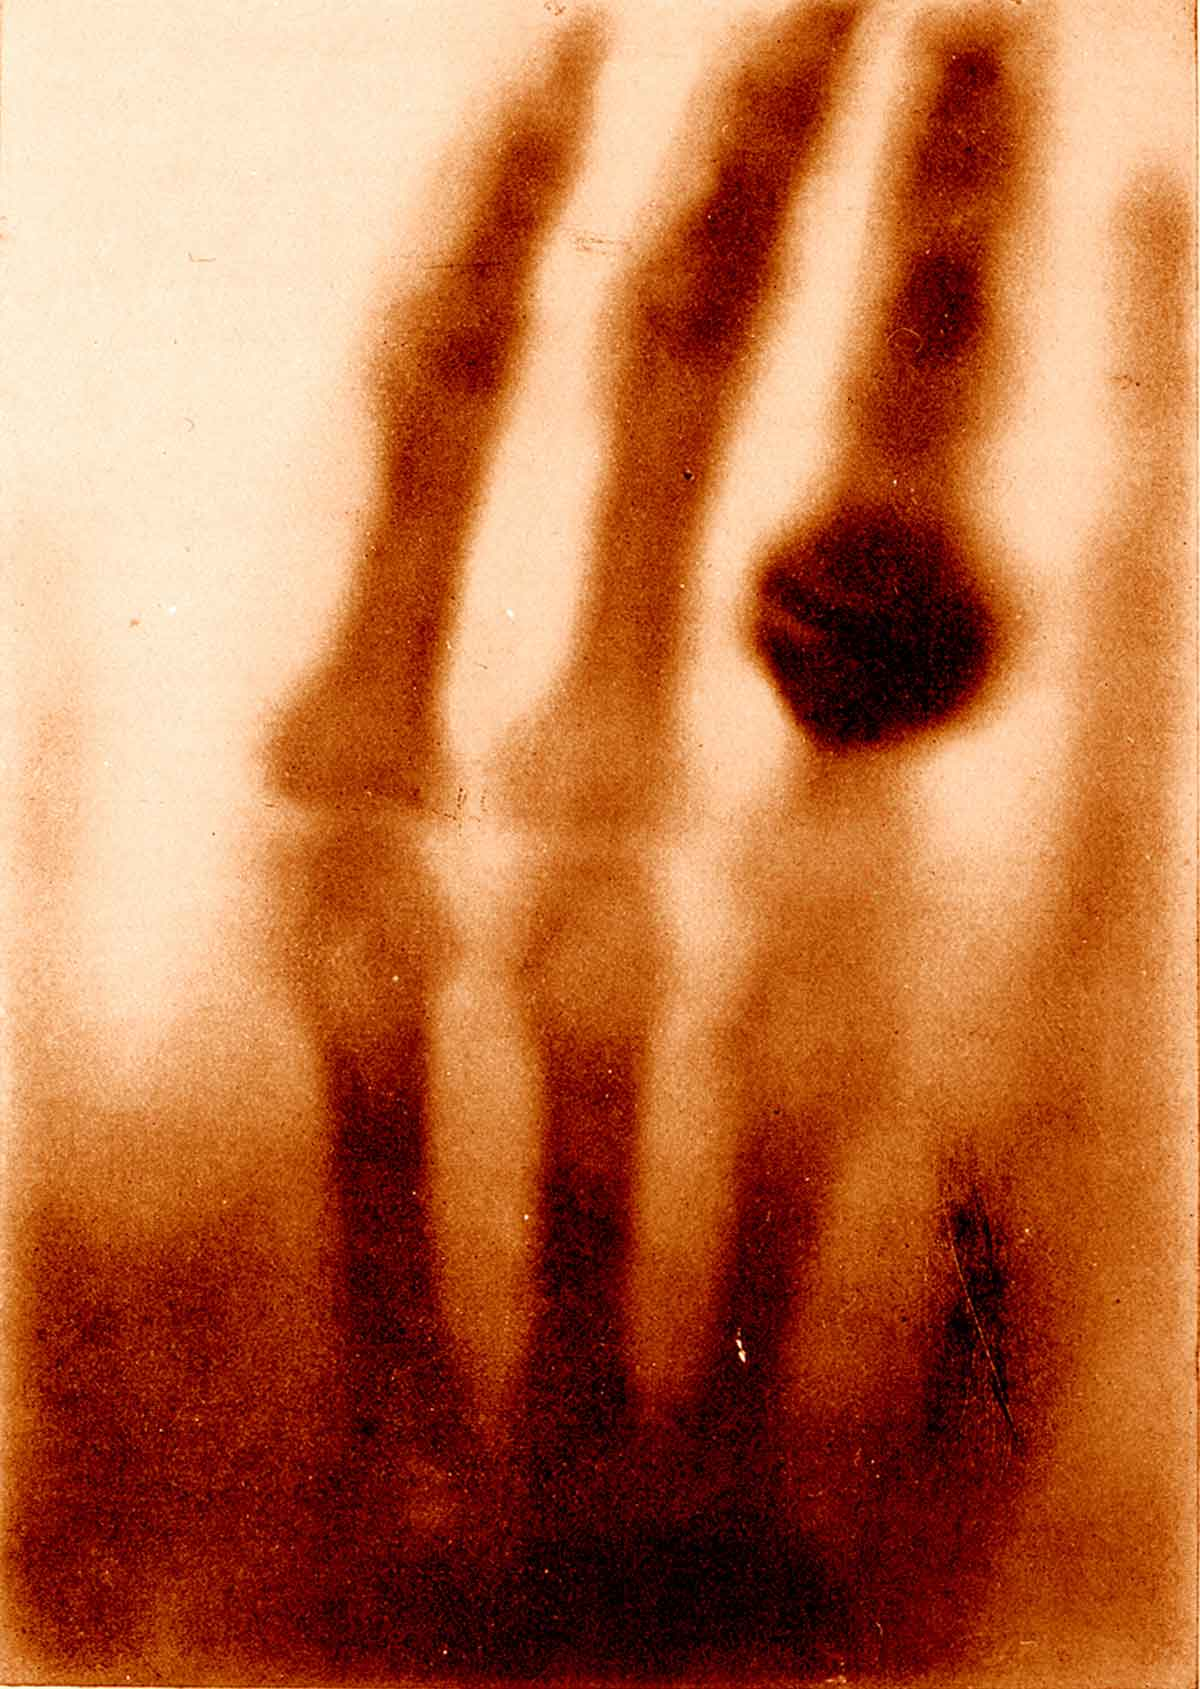
\includegraphics[width=150pt]{images/first-rtg.jpg}
    \caption[The hand of Mrs. Wilhelm Roentgen: the first X-ray image, 1895]{The hand of Mrs. Wilhelm Roentgen: the first X-ray image, 1895 \cite{glasser1993}}
    \label{fig:first-rtg}
\end{figure}

 Another important milestone in the medical field was ultrasound. Unlike X-Ray, ultrasound had been already used in other areas (localisation of submarines, detection of flaws in metals) before its introduction into medical diagnosis. Ultrasound is a high-frequency sound. So high, a human ear cannot detect it. A probe is used to transmit these waves into patient's body. The sound-waves echo from internal tissues and are reflected back to the probe. Then, an image representation is computed from the reflections. In 1958, Ian Donald and his team published the first paper about the use of ultrasound in obstetrics and gynaecology. They managed to get the first image of a fetus. Ultrasound gained popularity also due to its non-invasiveness and harmlessnes (in comparison to X-Rays). By 2000, modern real-time scanning machines with 3D/4D options were already available on the market.
 
 After 60 years from the invention of X-Rays, a biomedical engineer Godfrey Hounsfield came up with an idea to create three-dimensional scans of the human body. K. B. Bhattacharyya summarised Hounsfield's journey in his article \cite{bhattacharyya2016}: He wanted to develop a software that would compile X-Ray images from various angles into a 3D one. He succeeded and constructed the first CAT (computed axial tomography) scanner. In 1971, CAT scanners began to be used in hospitals. They could produce scans of brains, which was very helpful in diagnosing brain lesions. Hounsfield worked very hard to improve his inventions, so other parts of the body could be imaged as well. He was awarded a Nobel Prize for Medicine in 1979. I will talk more about C(A)T scans in the later chapters.
 
In 1973 we could witness another breakthrough in the medical imaging domain - MRI (magnetic resonance imaging). First, we need to go back to its roots in the 1930s. Austrian scientist Isidor Isaac Rabi discovered, that molecules passing through a magnetic field emit specific radio waves and change their spins. Each atom or molecule resonates with different frequencies that can be used to identify them and distinguish between types. This phenomenon is known as nuclear magnetic resonance (NMR). Paul Lauterbur found a way for NMR to produce images. He used the signals from different atoms to build the pictures \cite{lauterbur1973}. In contrast to X-Rays or CT, MRI does not emit radiation and is generally safer. MRI works well with soft tissues, for example brain.

Nowadays, all these imaging techniques (and others) are widely used and are a crucial part of the process of diagnosis and treatment. All the devices have been keeping up with the latest technology and are able to produce better results leading to more accurate diagnosis. Additionally, potential health risks from their use have been more thoroughly researched and reduced.

According to data from Eurostat \cite{eurostat2019}, the number of examinations by medical imaging techniques is still on a rise worldwide, as the technology is becoming more available. In Slovakia, there were 42,468 examinations performed using MRI in 1996. 20 years later it was 333,599. Similarly, the number of CT scans has grown 6-times in the same time period. Naturally, there was a need for image processing techniques that would either enhance some features of these images, make them more easily interpretable for doctors or even detect specific objects. Furthermore, we wanted to automatise these processes. 




 


